% Adapted from the downloaded IEEE conference template. IEEEtran.cls is unmodified.
\documentclass[conference]{IEEEtran}
\usepackage[T1]{fontenc}
\usepackage{cite}
\usepackage{amsmath,amssymb,amsfonts}
\usepackage{graphicx}
\usepackage{textcomp}
\usepackage{booktabs}
\usepackage{url}
\usepackage[hidelinks]{hyperref}
\hypersetup{pdftitle={An Empirical Study of Training and Post-Training Strategies for VGG16-GeM Image Retrieval},pdfauthor={Author 1, Author 2, Author 3}}
\graphicspath{{figures/}}
\newcommand{\Rone}{R1}
\newcommand{\Rtwo}{R2}
\newcommand{\checkpointrows}{%
B0 best & 12 & 81.06 & 77.12 \\
B0 last available & 14 & 80.77 & 76.08 \\
R1 best & 27 & 79.53 & 71.93 \\
R2 best & 28 & 80.49 & 72.76 \\
R1 final & 100 & 74.00 & 64.29 \\
R2 final & 100 & 71.37 & 62.72 \\%
}
\newcommand{\posttrainingrows}{%
Cosine & 74.00 & 70.80 & 64.29 & 62.84 & 71.37 & 68.15 & 62.72 & 61.59 \\
AQE & 76.41 & 73.81 & 65.90 & 64.84 & 73.64 & 70.86 & 64.06 & 63.36 \\
$\alpha$-QE & 76.45 & 73.86 & 65.89 & 64.83 & 73.63 & 70.90 & 64.06 & 63.36 \\
Gated QE & 76.45 & 73.86 & 65.89 & 64.83 & 73.63 & 70.90 & 64.06 & 63.36 \\
Local re-rank & 78.53 & 75.08 & 65.42 & 64.01 & 76.55 & 73.35 & 63.92 & 62.83 \\
Geometric re-rank & 76.68 & 73.46 & 64.83 & 63.40 & 74.98 & 71.84 & 63.33 & 62.19 \\
Verified QE & 78.94 & 76.28 & 66.97 & 65.82 & 76.85 & 74.25 & 65.10 & 64.31 \\
Mutual diffusion & 48.95 & 47.32 & 53.11 & 52.26 & 51.15 & 49.63 & 52.55 & 52.01 \\
Union diffusion & 23.67 & 22.10 & 45.61 & 45.15 & 25.79 & 24.13 & 46.15 & 46.05 \\%
}
\newcommand{\fusionrows}{%
Score fusion & 73.55 & 70.40 & 64.04 & 62.77 \\
RRF & 73.43 & 70.25 & 64.11 & 62.80 \\%
}
\newcommand{\sensitivityrows}{%
R1+R2 & Ox & RRF & c=100 & 73.41 \\
R1+R2 & Ox & RRF & c=10 & 73.56 \\
R1+R2 & Pa & RRF & c=100 & 64.08 \\
R1+R2 & Pa & RRF & c=10 & 64.13 \\
R1 & Ox & $\alpha$-QE & k=10, alpha=3, lam=0.25 & 75.58 \\
R1 & Ox & $\alpha$-QE & k=10, alpha=3, lam=1 & 77.30 \\
R1 & Ox & $\alpha$-QE & k=10, alpha=5, lam=0.5 & 76.54 \\
R1 & Ox & $\alpha$-QE & k=10, alpha=1, lam=0.5 & 76.42 \\
R1 & Ox & $\alpha$-QE & k=20, alpha=3, lam=0.5 & 75.52 \\
R1 & Ox & $\alpha$-QE & k=5, alpha=3, lam=0.5 & 77.15 \\
R1 & Ox & Mutual diffusion & k=40, beta=0.9 & 48.66 \\
R1 & Ox & Mutual diffusion & k=10, beta=0.9 & 55.91 \\
R1 & Ox & Mutual diffusion & k=20, beta=0.5 & 68.46 \\
R1 & Ox & Mutual diffusion & k=20, beta=0.99 & 28.16 \\
R1 & Ox & Union diffusion & k=40, beta=0.9 & 18.16 \\
R1 & Ox & Union diffusion & k=10, beta=0.9 & 29.12 \\
R1 & Ox & Union diffusion & k=20, beta=0.5 & 58.00 \\
R1 & Ox & Union diffusion & k=20, beta=0.99 & 8.43 \\
R1 & Ox & Gated QE & k=10, alpha=3, lam=0.5, tau=0.4 & 76.45 \\
R1 & Ox & Gated QE & k=10, alpha=3, lam=0.5, tau=0.6 & 76.45 \\
R1 & Ox & Geometric re-rank & k=50, eta=0.25 & 76.74 \\
R1 & Ox & Geometric re-rank & k=20, eta=0.5 & 74.86 \\
R1 & Ox & Geometric re-rank & k=50, eta=0.75 & 76.64 \\
R1 & Ox & Geometric re-rank & k=100, eta=0.5 & 77.37 \\
R1 & Ox & Local re-rank & k=50, eta=0.25 & 78.95 \\
R1 & Ox & Local re-rank & k=20, eta=0.5 & 75.99 \\
R1 & Ox & Local re-rank & k=50, eta=0.75 & 78.23 \\
R1 & Ox & Local re-rank & k=100, eta=0.5 & 78.85 \\
R1 & Pa & $\alpha$-QE & k=10, alpha=3, lam=0.25 & 65.27 \\
R1 & Pa & $\alpha$-QE & k=10, alpha=3, lam=1 & 66.56 \\
R1 & Pa & $\alpha$-QE & k=10, alpha=5, lam=0.5 & 65.89 \\
R1 & Pa & $\alpha$-QE & k=10, alpha=1, lam=0.5 & 65.90 \\
R1 & Pa & $\alpha$-QE & k=20, alpha=3, lam=0.5 & 65.86 \\
R1 & Pa & $\alpha$-QE & k=5, alpha=3, lam=0.5 & 65.71 \\
R1 & Pa & Mutual diffusion & k=40, beta=0.9 & 54.74 \\
R1 & Pa & Mutual diffusion & k=10, beta=0.9 & 49.36 \\
R1 & Pa & Mutual diffusion & k=20, beta=0.5 & 60.68 \\
R1 & Pa & Mutual diffusion & k=20, beta=0.99 & 41.93 \\
R1 & Pa & Union diffusion & k=40, beta=0.9 & 41.45 \\
R1 & Pa & Union diffusion & k=10, beta=0.9 & 46.28 \\
R1 & Pa & Union diffusion & k=20, beta=0.5 & 58.57 \\
R1 & Pa & Union diffusion & k=20, beta=0.99 & 20.59 \\
R1 & Pa & Gated QE & k=10, alpha=3, lam=0.5, tau=0.4 & 65.89 \\
R1 & Pa & Gated QE & k=10, alpha=3, lam=0.5, tau=0.6 & 65.89 \\
R1 & Pa & Geometric re-rank & k=50, eta=0.25 & 64.83 \\
R1 & Pa & Geometric re-rank & k=20, eta=0.5 & 64.44 \\
R1 & Pa & Geometric re-rank & k=50, eta=0.75 & 64.83 \\
R1 & Pa & Geometric re-rank & k=100, eta=0.5 & 65.55 \\
R1 & Pa & Local re-rank & k=50, eta=0.25 & 65.42 \\
R1 & Pa & Local re-rank & k=20, eta=0.5 & 64.55 \\
R1 & Pa & Local re-rank & k=50, eta=0.75 & 65.42 \\
R1 & Pa & Local re-rank & k=100, eta=0.5 & 66.94 \\
R2 & Ox & $\alpha$-QE & k=10, alpha=3, lam=0.25 & 72.96 \\
R2 & Ox & $\alpha$-QE & k=10, alpha=3, lam=1 & 74.32 \\
R2 & Ox & $\alpha$-QE & k=10, alpha=5, lam=0.5 & 73.64 \\
R2 & Ox & $\alpha$-QE & k=10, alpha=1, lam=0.5 & 73.63 \\
R2 & Ox & $\alpha$-QE & k=20, alpha=3, lam=0.5 & 72.48 \\
R2 & Ox & $\alpha$-QE & k=5, alpha=3, lam=0.5 & 74.01 \\
R2 & Ox & Mutual diffusion & k=40, beta=0.9 & 50.41 \\
R2 & Ox & Mutual diffusion & k=10, beta=0.9 & 56.04 \\
R2 & Ox & Mutual diffusion & k=20, beta=0.5 & 66.58 \\
R2 & Ox & Mutual diffusion & k=20, beta=0.99 & 29.29 \\
R2 & Ox & Union diffusion & k=40, beta=0.9 & 20.24 \\
R2 & Ox & Union diffusion & k=10, beta=0.9 & 30.51 \\
R2 & Ox & Union diffusion & k=20, beta=0.5 & 57.81 \\
R2 & Ox & Union diffusion & k=20, beta=0.99 & 9.14 \\
R2 & Ox & Gated QE & k=10, alpha=3, lam=0.5, tau=0.4 & 73.63 \\
R2 & Ox & Gated QE & k=10, alpha=3, lam=0.5, tau=0.6 & 73.63 \\
R2 & Ox & Geometric re-rank & k=50, eta=0.25 & 75.04 \\
R2 & Ox & Geometric re-rank & k=20, eta=0.5 & 73.48 \\
R2 & Ox & Geometric re-rank & k=50, eta=0.75 & 74.94 \\
R2 & Ox & Geometric re-rank & k=100, eta=0.5 & 75.68 \\
R2 & Ox & Local re-rank & k=50, eta=0.25 & 76.90 \\
R2 & Ox & Local re-rank & k=20, eta=0.5 & 74.18 \\
R2 & Ox & Local re-rank & k=50, eta=0.75 & 76.36 \\
R2 & Ox & Local re-rank & k=100, eta=0.5 & 77.29 \\
R2 & Pa & $\alpha$-QE & k=10, alpha=3, lam=0.25 & 63.55 \\
R2 & Pa & $\alpha$-QE & k=10, alpha=3, lam=1 & 64.63 \\
R2 & Pa & $\alpha$-QE & k=10, alpha=5, lam=0.5 & 64.06 \\
R2 & Pa & $\alpha$-QE & k=10, alpha=1, lam=0.5 & 64.07 \\
R2 & Pa & $\alpha$-QE & k=20, alpha=3, lam=0.5 & 64.33 \\
R2 & Pa & $\alpha$-QE & k=5, alpha=3, lam=0.5 & 64.10 \\
R2 & Pa & Mutual diffusion & k=40, beta=0.9 & 53.81 \\
R2 & Pa & Mutual diffusion & k=10, beta=0.9 & 50.17 \\
R2 & Pa & Mutual diffusion & k=20, beta=0.5 & 59.46 \\
R2 & Pa & Mutual diffusion & k=20, beta=0.99 & 41.94 \\
R2 & Pa & Union diffusion & k=40, beta=0.9 & 41.77 \\
R2 & Pa & Union diffusion & k=10, beta=0.9 & 46.51 \\
R2 & Pa & Union diffusion & k=20, beta=0.5 & 58.14 \\
R2 & Pa & Union diffusion & k=20, beta=0.99 & 20.03 \\
R2 & Pa & Gated QE & k=10, alpha=3, lam=0.5, tau=0.4 & 64.06 \\
R2 & Pa & Gated QE & k=10, alpha=3, lam=0.5, tau=0.6 & 64.06 \\
R2 & Pa & Geometric re-rank & k=50, eta=0.25 & 63.33 \\
R2 & Pa & Geometric re-rank & k=20, eta=0.5 & 62.85 \\
R2 & Pa & Geometric re-rank & k=50, eta=0.75 & 63.33 \\
R2 & Pa & Geometric re-rank & k=100, eta=0.5 & 64.24 \\
R2 & Pa & Local re-rank & k=50, eta=0.25 & 63.93 \\
R2 & Pa & Local re-rank & k=20, eta=0.5 & 62.99 \\
R2 & Pa & Local re-rank & k=50, eta=0.75 & 63.92 \\
R2 & Pa & Local re-rank & k=100, eta=0.5 & 65.55 \\%
}
\newcommand{\secondaryrows}{%
R1+R2 & Ox & RRF & 79.66 & 48.98 & 67.05 & 77.00 & 50.83 \\
R1+R2 & Ox & score\_fusion & 79.92 & 48.92 & 67.05 & 77.07 & 50.93 \\
R1+R2 & Pa & RRF & 91.68 & 13.93 & 30.05 & 48.78 & 55.16 \\
R1+R2 & Pa & score\_fusion & 91.72 & 13.94 & 30.07 & 48.80 & 55.25 \\
R1 & Ox & AQE & 81.05 & 50.96 & 68.79 & 78.68 & 55.28 \\
R1 & Ox & $\alpha$-QE & 81.11 & 50.98 & 68.80 & 78.67 & 55.32 \\
R1 & Ox & Cosine & 79.21 & 48.98 & 66.88 & 77.30 & 48.33 \\
R1 & Ox & Mutual diffusion & 67.70 & 34.32 & 47.92 & 58.71 & 37.96 \\
R1 & Ox & Union diffusion & 29.77 & 8.89 & 20.35 & 32.58 & 13.46 \\
R1 & Ox & Gated QE & 81.11 & 50.98 & 68.80 & 78.67 & 55.32 \\
R1 & Ox & Geometric re-rank & 82.65 & 50.67 & 66.88 & 77.30 & 54.17 \\
R1 & Ox & Local re-rank & 84.22 & 52.34 & 66.88 & 77.30 & 55.96 \\
R1 & Ox & Verified QE & 83.58 & 52.70 & 69.83 & 79.41 & 60.97 \\
R1 & Pa & AQE & 92.26 & 14.13 & 30.33 & 50.13 & 58.17 \\
R1 & Pa & $\alpha$-QE & 92.27 & 14.13 & 30.33 & 50.12 & 58.17 \\
R1 & Pa & Cosine & 91.18 & 13.90 & 29.59 & 48.74 & 54.71 \\
R1 & Pa & Mutual diffusion & 88.32 & 13.36 & 27.88 & 42.15 & 46.49 \\
R1 & Pa & Union diffusion & 69.08 & 9.87 & 21.04 & 35.19 & 40.68 \\
R1 & Pa & Gated QE & 92.27 & 14.13 & 30.33 & 50.12 & 58.17 \\
R1 & Pa & Geometric re-rank & 94.40 & 14.28 & 29.59 & 48.74 & 55.13 \\
R1 & Pa & Local re-rank & 96.41 & 14.90 & 29.59 & 48.74 & 55.67 \\
R1 & Pa & Verified QE & 94.17 & 14.37 & 30.73 & 50.70 & 58.60 \\
R2 & Ox & AQE & 79.81 & 49.28 & 66.89 & 77.32 & 57.29 \\
R2 & Ox & $\alpha$-QE & 79.86 & 49.31 & 66.93 & 77.33 & 57.35 \\
R2 & Ox & Cosine & 78.66 & 48.07 & 65.45 & 75.69 & 50.91 \\
R2 & Ox & Mutual diffusion & 69.15 & 35.77 & 51.19 & 59.94 & 42.50 \\
R2 & Ox & Union diffusion & 30.02 & 10.28 & 22.74 & 38.98 & 15.59 \\
R2 & Ox & Gated QE & 79.86 & 49.31 & 66.93 & 77.33 & 57.35 \\
R2 & Ox & Geometric re-rank & 82.70 & 49.73 & 65.45 & 75.69 & 56.83 \\
R2 & Ox & Local re-rank & 83.85 & 51.32 & 65.45 & 75.69 & 57.68 \\
R2 & Ox & Verified QE & 82.87 & 51.49 & 68.88 & 78.35 & 60.88 \\
R2 & Pa & AQE & 92.49 & 14.08 & 30.58 & 49.48 & 57.70 \\
R2 & Pa & $\alpha$-QE & 92.52 & 14.08 & 30.57 & 49.48 & 57.70 \\
R2 & Pa & Cosine & 91.71 & 13.89 & 29.87 & 48.28 & 54.40 \\
R2 & Pa & Mutual diffusion & 88.25 & 13.15 & 27.72 & 41.88 & 47.38 \\
R2 & Pa & Union diffusion & 70.19 & 10.21 & 22.05 & 36.69 & 42.74 \\
R2 & Pa & Gated QE & 92.52 & 14.08 & 30.57 & 49.48 & 57.70 \\
R2 & Pa & Geometric re-rank & 94.71 & 14.32 & 29.87 & 48.28 & 54.77 \\
R2 & Pa & Local re-rank & 96.31 & 15.05 & 29.87 & 48.28 & 55.11 \\
R2 & Pa & Verified QE & 94.40 & 14.30 & 30.99 & 50.04 & 57.75 \\%
}

\newcommand{\revisiondiffusionrows}{%
R1 & 77.46 & 76.21 & 77.26 & 76.34 \\
R2 & 73.80 & 72.45 & 77.79 & 77.06 \\%
}
\newcommand{\revisionbaselinerows}{%
Cosine & 81.06 & 78.77 & 77.13 & 75.63 \\
AQE & 83.77 & 82.22 & 80.19 & 79.07 \\
$\alpha$-QE & 83.76 & 82.25 & 80.17 & 79.05 \\
Gated QE & 83.76 & 82.25 & 80.17 & 79.05 \\
Sparse diffusion & 78.35 & 77.46 & 90.50 & 89.16 \\%
}

\begin{document}
\title{An Empirical Study of Training and Post-Training Strategies for VGG16--GeM Image Retrieval}
\author{\IEEEauthorblockN{Author 1 \qquad Author 2 \qquad Author 3}}
\maketitle
\begin{abstract}
We examine checkpoint selection and search-time processing in a VGG16--GeM image-retrieval pipeline trained with structure-from-motion supervision. The study combines historical augmentation and spatial-gate runs with a completed evaluation of the validation-selected B0 checkpoint on legacy Oxford5k and Paris6k. Five fixed search methods are tested on clean queries and six corruption families at three severity levels, producing 17,050 B0 per-query AP records. Average query expansion raises B0 corrupted dataset-macro mAP from 77.20 to 80.64 percent. An implementation audit also explains a severe archived diffusion failure: dense query seeds give 23.67 percent clean mAP on the R1 Oxford union graph, while fixed top-20 seeds recover 76.75 percent on that same graph. On B0, mutual/top-20 diffusion reaches 83.31 percent corrupted dataset-macro mAP, but its effect differs by dataset: clean Oxford falls from 81.06 to 78.35 percent, whereas Paris rises from 77.13 to 90.50 percent. The two historical fine-tuned runs show late-training validation deterioration; neither establishes a consistent training improvement over B0. Archived geometry-verified expansion improves their rankings at a seconds-per-query cost. Together, the results identify checkpoint choice, feedback quality and diffusion initialization as practical determinants of retrieval performance. Published source, numerical outputs, input hashes and independent solver checks support reproducing the measurements.
\end{abstract}
\begin{IEEEkeywords}
instance image retrieval, generalized-mean pooling, query expansion, geometric verification, robustness evaluation
\end{IEEEkeywords}
\section{Introduction}
Instance image retrieval ranks gallery images depicting the same particular object or landmark as a query. A global descriptor enables inexpensive similarity search, but its usefulness depends on both the learned representation and the processing applied after the initial ranking. Fine-tuning can adapt a classification backbone to retrieval, while query expansion, local verification, fusion, and graph propagation offer additional ways to alter rankings without updating encoder weights.

The VGG16--GeM pipeline provides an established setting for examining these choices. VGG networks supply convolutional representations~\cite{vgg}, and generalized-mean pooling (GeM) supports compact descriptors learned from structure-from-motion (SfM) supervision~\cite{gem}. However, adding augmentation, attention, or more epochs does not by itself establish an improvement. Likewise, a search method that helps a fixed final checkpoint need not outperform a stronger historical checkpoint. Mixing these comparisons can obscure what an experiment actually demonstrates.

We examine three available training histories: a baseline reproduction, denoted B0, an augmentation-only run (\Rone), and an augmentation-plus-spatial-gate run (\Rtwo). The training comparison is historical rather than a fully controlled ablation. We separately conduct a fixed-encoder search study using the two new epoch-100 checkpoints, re-extracted with the same FP32 inference protocol. A third evaluation applies five fixed methods to validation-selected B0 on both clean and corrupted queries, so search conclusions also include the stronger baseline checkpoint.

Our study addresses three questions. \emph{RQ1:} How do validation-selected and final checkpoints compare, and what evidence supports the training modifications? \emph{RQ2:} Which post-training methods improve clean and corrupted-query retrieval for the same fixed encoder? \emph{RQ3:} How much query-time computation is required for these gains?

The contributions are empirical: (1) an audit of training configuration, data splits, and checkpoint selection; (2) a four-family search study for two final encoders, extended by a five-method clean/robustness evaluation of validation-selected B0; and (3) a comparison of retrieval-only and direct end-to-end latency, retaining unsuccessful methods and exploratory sensitivity results. The work evaluates combinations of established components; it does not introduce a new pooling, attention, or geometric-verification algorithm.

\section{Related Work}
\subsection{Learned Global Representations}
Radenovi\'{c} \emph{et al.} use SfM reconstructions to obtain matching and non-matching training examples without manual retrieval labels, and introduce trainable GeM pooling~\cite{gem}. We adopt this descriptor-learning framework on a prepared subset, retaining a single global descriptor and disabling whitening and multi-scale inference. Our results therefore should not be interpreted as a reproduction of every component or headline score of the original system.

Spatial attention is another way to alter feature aggregation. CBAM combines channel and spatial attention~\cite{cbam}. Our second run uses only a small spatial gate inspired by channel-mean and channel-max aggregation, with identity-preserving initialization and a scaled sigmoid. It is not a full CBAM implementation.

Modern visual backbones broaden the representation choices. Vision Transformer (ViT) processes images as sequences of patches~\cite{vit}, while DINOv2 learns transferable visual features through large-scale self-supervision~\cite{dinov2}. These approaches provide relevant alternatives to the convolutional encoder studied here. Our VGG16 experiments examine checkpoint selection and search processing within one established descriptor family; they do not rank modern backbones.

\subsection{Feedback, Geometry, and Ranking}
Visual query expansion uses initially retrieved images to refine the query. Chum \emph{et al.} combine feedback with spatial verification to limit false-positive expansion~\cite{totalrecall}. We evaluate descriptor-level averaging, similarity weighting, a cosine gate, and a geometry-filtered feedback pipeline. RootSIFT applies a normalization and square-root transformation to local SIFT descriptors~\cite{rootsift}; it supplies the local evidence in our re-ranking and verification stages. Homographies are estimated using RANSAC~\cite{ransac}.

Reciprocal rank fusion (RRF) combines rank positions rather than requiring matching score scales~\cite{rrf}. Diffusion can exploit neighborhood structure; Iscen \emph{et al.} study propagation over regional CNN representations~\cite{diffusion}. Our graph is built from one global descriptor per gallery image, so a failure here is not evidence against their regional method.

DELG unifies learned local and global features in one network, combining GeM-based global retrieval with attentive local representations~\cite{delg}. SuperGlobal instead refines global representations for both retrieval and re-ranking~\cite{superglobal}. Together they motivate evaluating the cost of local matching against global-only feedback. Our RootSIFT verification and residual QE are simpler reference pipelines, with their storage and query costs measured explicitly.

\subsection{Benchmark Protocols}
Oxford and Paris originate from landmark-retrieval research~\cite{oxford,paris}. Revised annotations and evaluation protocols were subsequently introduced~\cite{revisited}. We use the available \emph{legacy} ground truth with 55 queries per dataset. Results are consequently not interchangeable with revisited Easy, Medium, or Hard scores. Our corruption suite is a deterministic extension of these query images, not a newly annotated independent benchmark.

\section{Methods}
\subsection{Encoder and Tuple Objective}
For nonnegative convolutional activations $x_{c,u}$ at channel $c$ and position $u\in\mathcal U$, GeM computes
\begin{equation}
 g_c=\left(\frac{1}{|\mathcal U|}\sum_{u\in\mathcal U}x_{c,u}^{p}\right)^{1/p},
 \qquad \mathbf z=\frac{\mathbf g}{\|\mathbf g\|_2}.
\end{equation}
A shared learnable $p$ starts at 3. VGG16 features, without the classifier and final pooling, produce a 512-dimensional normalized descriptor. The initial ranking uses cosine score $s_i=\mathbf z_q^\top\mathbf z_i$.

Each training tuple contains a query $q$, one metadata-defined positive $p$, and five negatives $n_j$. The implemented objective is
\begin{equation}
 \mathcal L=\tfrac12 d(q,p)^2+\tfrac12\sum_{j=1}^{5}[m-d(q,n_j)]_+^2,
 \quad m=0.7,
\end{equation}
where $[a]_+=\max(a,0)$ and $d$ is Euclidean descriptor distance. The implementation adds $10^{-6}$ to coordinate differences before computing the norm for numerical stabilization. Positive relations come from explicit metadata pairs; cluster membership alone does not assign a positive label. Hard-negative mining uses current clean descriptors, excludes the query cluster, and selects negatives from distinct clusters.

\subsection{Training Modifications}
\Rone{} adds independent photometric and degradation transforms to the images used in the training forward pass. With probability 0.8, brightness and contrast factors are drawn from $[0.8,1.2]$ and color from $[0.85,1.15]$, in random order. Gaussian blur is applied with probability 0.15 and radius $[0.2,1.0]$ pixels; JPEG encoding with probability 0.2 and integer quality 55--95; and erasing with probability 0.15, area 1--5\%, and aspect ratio 0.5--2. Erasing fills zero after normalization, corresponding to the normalization mean in RGB. Clean mining and validation do not use these transforms.

\Rtwo{} adds a spatial gate before GeM. For feature tensor $X$, the gate is
\begin{equation}
 A(X)=2\sigma\!\left(\operatorname{Conv}_{7\times7}
 [\operatorname{mean}_cX;\operatorname{max}_cX]\right).
\end{equation}
The two-input, one-output convolution has 99 parameters including bias. Zero-initialized weights and bias give $A(X)=1$, so the initial gated tensor equals $X$. The output descriptor dimensionality remains unchanged.

\subsection{Query Expansion and Feedback Selection}
Let $\mathcal F$ be positive-cosine candidates from the first top-$k$ ranking. We compute
\begin{equation}
 \mathbf q'=\operatorname{norm}_2\!\left(\mathbf q+
 \lambda\frac{\sum_{i\in\mathcal F}w_i\mathbf z_i}{\sum_{i\in\mathcal F}w_i}\right),
 \quad w_i=\max(s_i,0)^\alpha .
 \label{eq:qe}
\end{equation}
AQE uses $\alpha=0$; weighted QE uses $\alpha=3$. We fix $k=10$ and $\lambda=0.5$ for one feedback iteration. Gated QE additionally requires $s_i\geq0.5$ and at least three accepted candidates, otherwise returning the original query. Setting $\lambda=0$ also returns the baseline. The residual form in~\eqref{eq:qe} is stated explicitly because conventions for mixing query and feedback differ.

\subsection{Local and Geometric Evidence}
We extract up to 2,000 RootSIFT keypoints per image. Matching uses a 0.75 nearest-neighbor ratio test and mutual nearest-neighbor consistency. Homography RANSAC uses a 3-pixel threshold, confidence 0.995, and at most 2,000 iterations. A valid result requires at least eight inliers and a finite, full-rank homography with condition number below $10^{12}$.

For a top-50 candidate with $M_i$ matches and $I_i$ inliers, local re-ranking uses evidence $e_i=\min(M_i/50,1)$. Geometric re-ranking instead uses
\begin{equation}
 e_i=\frac{I_i}{\max(M_i,1)}\min(I_i/20,1)
\end{equation}
when geometry is valid, and zero otherwise. The combined score is $(1-\eta)(s_i+1)/2+\eta e_i$, with $\eta=0.5$. Only the candidate prefix changes; the remaining ranking is retained. Invalid query features or no valid geometric candidate trigger a logged fallback where applicable.

\emph{Verified QE} checks the first 50 global candidates, selects at most ten with valid geometry and positive cosine, and applies~\eqref{eq:qe}. Fewer than three valid feedback images returns the original query. Search is then repeated over the entire gallery, without a second re-ranking stage. Relevance and junk labels never select feedback.

\subsection{Fusion and Diffusion}
Score fusion averages the two encoders' cosine scores after image-ID alignment. RRF uses both full rankings:
\begin{equation}
 S_{\mathrm{RRF}}(i)=\sum_{r=1}^{2}\frac{1}{60+\operatorname{rank}_r(i)}.
\end{equation}
We do not average raw embeddings across encoders.

Each encoder also defines a gallery graph with $k=20$, no self-edges, and directed weights $\max(s_{ij},0)^3$. Union and mutual graphs use the elementwise maximum and minimum with the transposed affinity, respectively. Let $S=D^{-1/2}WD^{-1/2}$, using zero inverse degree for isolated nodes. Initial query scores $y_i$ are positive-cosine cubes normalized to unit sum. We iterate
\begin{equation}
 \mathbf f^{(t+1)}=(1-\beta)\mathbf y+\beta S\mathbf f^{(t)},
 \quad \beta=0.9,
\end{equation}
starting at $\mathbf f^{(0)}=\mathbf y$, stopping at relative L2 change below $10^{-6}$ or 100 iterations. Non-finite results or absent initial mass fall back to cosine. Labels are not used in graph construction or propagation.

\section{Experimental Setup}
\subsection{Training Data and Validation}
The prepared SfM subset contains 15,953 training images from 100 clusters and 34,337 explicit query--positive pairs. Validation contains 739 images from 20 clusters and 181 pairs. Image identifiers and clusters are disjoint between these partitions. We have not established semantic landmark disjointness between SfM and the retrieval benchmarks.

Each epoch samples 2,000 training tuples. The requested mining pool of 20,000 is clipped to the 15,953 available training images. Thus, an epoch does not enumerate all positive pairs. Five tuple losses are summed before each Adam update, giving 400 updates per epoch. Although each update contains 35 image positions, duplicate images are possible. The microbatch limit of eight applies only to same-shape forward groups; it does not change the optimizer's five-tuple batch. Tuple fusion is one in the new runs.

Validation uses no augmentation or gradient updates. With batch size five and the final incomplete batch dropped, 180 of the 181 validation tuples are processed. For the two new runs, validation pair sampling is seeded consistently, but mined negatives still depend on the current encoder. The selection criterion is validation contrastive loss, not benchmark mAP. Pair metadata alone does not provide exhaustive relevance labels for a retrieval development set.

\begin{table}[t]
\caption{Training configuration. LR denotes base learning rate before scheduling. B0 is a historical reproduction.}
\label{tab:train}
\centering\footnotesize
\begin{tabular}{lcc}
\toprule
Setting & B0 & \Rone{} / \Rtwo{} \\
\midrule
Optimizer & Adam & Adam \\
Backbone LR & $10^{-6}$ & $10^{-6}$ \\
GeM LR & $10^{-5}$ & $10^{-5}$ \\
Gate LR & --- & --- / $10^{-4}$ \\
Backbone weight decay & $10^{-6}$ & $10^{-6}$ \\
GeM / gate weight decay & 0 / --- & 0 / 0 \\
Training seed & 42 & 42 \\
Image long-edge cap & 1024 & 1024 \\
Tuples / update & 5 & 5 \\
Negatives / tuple & 5 & 5 \\
Completed epochs & 14 & 100 / 100 \\
Backbone train precision & FP32 & BF16 autocast \\
\bottomrule
\end{tabular}
\end{table}

\subsection{Optimization and Checkpoint Identity}
Table~\ref{tab:train} summarizes the settings. Adam~\cite{adam} uses a pre-epoch schedule $\mathrm{LR}(e)=\mathrm{LR}_0\exp(-0.01e)$, beginning at $e=1$. The new runs retain FP32 for GeM, descriptor normalization, loss, weights, and Adam state. They use four workers, extraction window eight, prefetch factor two, and no image cache. Training uses Colab; the new runs were configured for an A100 40-GB GPU. Runtime differences prevent an algorithm-only speed comparison with B0.

We distinguish three evidence tracks. The \emph{historical checkpoint comparison} uses saved clean evaluations: B0 best at epoch 12 and last available at 14, \Rone{} best at 27, and \Rtwo{} best at 28. The archived new-run best evaluations use BF16 backbone inference. The \emph{post-training comparison} uses both latest epoch-100 checkpoints, re-extracted in FP32 with TF32 disabled. The completed B0 study applies five fixed search methods to its validation-selected epoch-12 checkpoint, using the same query-corruption schedule and FP32 inference with TF32 disabled. B0 historical evaluations are also FP32; archived clean checkpoint scores remain separate from the new inference results.

The \Rone{} epoch-27 weight file is absent from the supplied archive, although its saved evaluation and history remain available. Its clean scores are reported as historical evidence, not as a newly repeated inference. Both final checkpoints and the B0 best checkpoint are available. Archive, source-checkpoint, exported-weight, and metadata hashes identify the inputs; exported final weights were checked against the source model before extraction.

\subsection{Retrieval Protocol and Corruptions}
Oxford5k contains 5,063 gallery images and Paris6k 6,392, each with 55 query regions. We retain the legacy bounding boxes, relevant-image labels, junk handling, and trapezoidal AP evaluator. Image-source queries may also occur in the gallery. AP is averaged over queries to form mAP. We additionally retain P@10 and relevant Recall@20/50/100 after junk removal. These are legacy scores, not revisited-protocol results~\cite{revisited}.

Inference uses one scale and no whitening. RGB images preserve aspect ratio under a long-edge cap of 1024. Query crops retain the upstream relative-resize rule: their cap is scaled by the ratio of crop to original long edge, rather than enlarging every crop to 1024. Values in $[0,1]$ are normalized by mean $(0.485,0.456,0.406)$ and standard deviation $(0.229,0.224,0.225)$.

\begin{table}[t]
\caption{Query corruptions at severities 1/2/3. $L$ is the resized query long edge; the gallery stays clean.}
\label{tab:corrupt}
\centering\footnotesize
\begin{tabular}{lp{0.56\columnwidth}}
\toprule
Family & Severity parameters \\
\midrule
Darkening & RGB factors 0.8 / 0.6 / 0.4 \\
Contrast & Factors about channel mean: 0.8 / 0.6 / 0.4 \\
Blur & Gaussian $\sigma/L$: 0.001 / 0.002 / 0.004 \\
Noise & Gaussian RGB std.: 0.02 / 0.05 / 0.08 \\
JPEG & Quality 80 / 50 / 25; subsampling 2 \\
Occlusion & Area fractions 0.05 / 0.10 / 0.20; query RGB-mean fill \\
\bottomrule
\end{tabular}
\end{table}

Corruptions in Table~\ref{tab:corrupt} are applied after crop/resize and before normalization. Blur uses a minimum sigma of 0.1 pixels. Noise and occlusion each have three fixed realizations per severity; other families have one. This produces 30 corrupted views plus clean per query: 3,410 query instances per encoder, or 6,820 forwards in the original two-encoder study. The completed B0 study uses those same 3,410 query instances, and all pixel checksums match the saved R1 inputs. Corruption seed 20261030 is independent of training seed 42. Pixel checksums enforce consistency between global and local features. Noise is absent from the training augmentation; the remaining families overlap in part but differ in generation or strength.

For $C=18$ family--severity conditions and their realization counts $R_c$, we report
\begin{equation}
 \mathrm{mAP}_{\mathrm{corr}}=\frac1C\sum_{c=1}^{C}
 \frac{1}{R_c}\sum_{r=1}^{R_c}\mathrm{mAP}_{c,r}.
\end{equation}
Dataset-macro results average Oxford and Paris equally. Worst-condition mAP is the minimum of the 18 realization-averaged condition scores. Drop is clean minus corrupted mAP in percentage points. Repeated views of the same query are not independent training replications.

\subsection{Frozen Parameters, Sensitivity, and Cost}
Main parameters are fixed across datasets and corruption conditions. Clean-only, one-axis sensitivity varies QE $k\in\{5,10,20\}$, $\alpha\in\{1,3,5\}$, $\lambda\in\{0.25,0.5,1\}$, gate $\tau\in\{0.4,0.5,0.6\}$; re-ranking $K\in\{20,50,100\}$ and $\eta\in\{0.25,0.5,0.75\}$; RRF $c\in\{10,60,100\}$; and diffusion $k\in\{10,20,40\}$ and $\beta\in\{0.5,0.9,0.99\}$. Main settings supply the reference, with 100 additional model--method--configuration--dataset rows. No separate labeled retrieval development set is available. We call all search results exploratory and do not promote a sensitivity maximum to the main configuration.

The original FP32 extraction used a Kaggle Tesla T4, PyTorch 2.11.0+cu128, NumPy 2.1.3 and Pillow 13.0.0. The completed B0 run used a Tesla T4 with PyTorch 2.11.0+cu130, the same NumPy/Pillow versions and OpenCV 4.14.0. It finished its measured work in 1,594.45 seconds, reusing verified Oxford gallery and clean-query descriptors; this is not a from-scratch extraction time or an online latency benchmark. Local processing used OpenCV 4.14.0; CPU jobs used SciPy 1.16.3. CPU allocation can differ between Kaggle jobs, so timings describe the measured deployment rather than a hardware-normalized algorithm benchmark.

Retrieval-only latency assumes cached descriptors. Direct end-to-end latency includes decoding, query crop/resize, corruption when applicable, encoding, search, and query local extraction/matching for local methods. Gallery descriptors, gallery local features, and graphs are offline assets. Timing uses batch one, warm-up, and GPU synchronization. For each model/dataset/method, 28 samples cover clean and severity-three queries from all six families, with two queries per condition and two repeats. Across 40 groups, this gives 1,120 direct samples. We report medians and retain p95 in the released tables; independently measured medians are not additive component costs.

\section{Results and Discussion}
\subsection{RQ1: Checkpoint Selection and Training Changes}
\begin{table}[t]
\caption{Historical clean mAP (\%). Best means minimum validation loss. R1/R2 best use archived BF16-backbone evaluations; final rows are the new FP32 cosine baselines.}
\label{tab:checkpoints}
\centering\footnotesize
\begin{tabular}{lrrr}
\toprule
Checkpoint & Epoch & Oxford & Paris \\
\midrule
\checkpointrows
\bottomrule
\end{tabular}
\end{table}

B0 best remains strongest on both clean benchmarks (Table~\ref{tab:checkpoints}), reaching 81.06\% on Oxford and 77.12\% on Paris. The best available historical evaluations for \Rone{} reach 79.53\% and 71.93\%; \Rtwo{} reaches 80.49\% and 72.76\%. The gate run is higher at these selected checkpoints, but this ordering reverses at epoch 100. Thus, the saved evidence does not support an unconditional benefit from the gate or superiority of either new run over B0.

\begin{figure*}[t]
\centering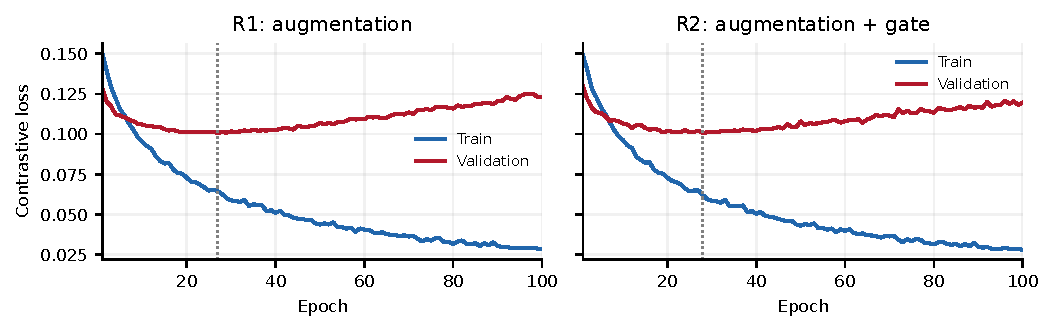
\includegraphics[width=0.92\textwidth]{training.pdf}
\caption{Training and validation contrastive loss for the two new runs. Dotted lines mark validation-selected epochs 27 and 28. Validation negatives depend on the current encoder; curves show the implemented monitoring objective.}
\label{fig:training}
\end{figure*}

The histories show late-training deterioration (Fig.~\ref{fig:training}). \Rone{} has minimum validation loss 0.100764 at epoch 27, rising to 0.123108 at epoch 100; \Rtwo{} rises from 0.100519 at epoch 28 to 0.119673. Meanwhile, training loss falls to approximately 0.0288 and 0.0280. Combined with lower final retrieval scores, this is consistent with overfitting. It does not isolate a single cause: optimization trajectory, augmentation, and changed precision/runtime are not independently controlled.

The archived B0 best epoch is 12, selected by validation, not by taking the best score separately on each benchmark. For example, B0's Paris score at epoch 8 is higher than at epoch 12, but substituting it would mix selection criteria. We preserve the declared checkpoint rule. Similarly, a lower validation loss across two runs is not automatically a calibrated estimate of better retrieval, particularly with changing mined negatives.

\subsection{RQ2: Search Improvements for Fixed Encoders}
\begin{table*}[t]
\caption{Main post-training results, mAP (\%). C denotes clean and R the mean over 18 corrupted-query conditions. Both encoders are fixed at epoch 100 and use FP32 extraction. These are exploratory comparisons against each encoder's own cosine baseline.}
\label{tab:post}
\centering\small
\begin{tabular}{lrrrrrrrr}
\toprule
& \multicolumn{4}{c}{\Rone{}: augmentation} & \multicolumn{4}{c}{\Rtwo{}: augmentation + gate} \\
\cmidrule(lr){2-5}\cmidrule(lr){6-9}
& \multicolumn{2}{c}{Oxford5k} & \multicolumn{2}{c}{Paris6k} & \multicolumn{2}{c}{Oxford5k} & \multicolumn{2}{c}{Paris6k} \\
Method & C & R & C & R & C & R & C & R \\
\midrule
\posttrainingrows
\bottomrule
\end{tabular}
\end{table*}

\paragraph{Expansion provides low-cost gains}
AQE and weighted QE improve both clean and corrupted mAP for both final encoders (Table~\ref{tab:post}). For \Rone, weighted QE increases Oxford clean from 74.00\% to 76.45\% and Paris clean from 64.29\% to 65.89\%. Equal-dataset corrupted mAP rises from 66.82\% to 69.34\%, a 2.52-percentage-point gain. AQE and weighted QE differ little, so these observations do not establish the necessity of similarity weighting.

The cosine gate opens for every measured query view and accepts ten feedback images, causing gated QE to equal weighted QE. This diagnostic is important: identical scores here indicate an inactive selection constraint, rather than evidence that the gate improves feedback reliability.

\paragraph{Geometry is most useful as a feedback filter}
For \Rone, local-match re-ranking reaches 78.53\% Oxford clean, exceeding the geometric-score re-ranker at 76.68\%. Geometric verification is therefore not uniformly stronger when used only to reorder a short prefix. In contrast, verified QE reaches 78.94\% and 66.97\% clean on Oxford and Paris, and 76.28\% and 65.82\% under corruption. Its corrupted dataset-macro mAP is 71.05\%, or 4.23 points above cosine. For \Rtwo, verified QE also gives the highest main-method mAP in all four columns: 76.85\%, 74.25\%, 65.10\%, and 64.31\%.

Verified feedback is not always available. Across clean and corrupted views, its gate opens for 88.39\% of \Rone{} Oxford cases and 92.96\% of Paris cases. The mean feedback counts, including closed gates, are 6.87 and 8.56. Fallbacks are retained rather than removing difficult queries from evaluation. These observations support examining feedback quality, but do not prove that the chosen homography criterion is optimal.

\begin{table}[t]
\caption{Two-encoder fusion, mAP (\%). Both use R1+R2 epoch 100; column order matches Table~\ref{tab:post}.}
\label{tab:fusion}
\centering\footnotesize
\begin{tabular}{lrrrr}
\toprule
& \multicolumn{2}{c}{Oxford} & \multicolumn{2}{c}{Paris} \\
Method & C & R & C & R \\
\midrule
\fusionrows
\bottomrule
\end{tabular}
\end{table}

\paragraph{Fusion does not beat the stronger encoder}
Neither score fusion nor RRF exceeds \Rone{} cosine on either clean dataset or their corrupted means (Table~\ref{tab:fusion}). Score fusion obtains 73.55\% Oxford clean and 64.04\% Paris clean, compared with 74.00\% and 64.29\% for \Rone. Complementary errors are a possible requirement for useful fusion, but we have not isolated error dependence as the cause. The experiment only establishes that these two encoders and combination rules do not improve the stronger single ranking.

\paragraph{Global graph diffusion degrades ranking}
Mutual diffusion reduces \Rone{} Oxford clean from 74.00\% to 48.95\%, and union diffusion to 23.67\%. Paris also deteriorates. This is not primarily explained by numerical failure: aggregate diagnostics report full convergence for both \Rone{} graphs, zero fallback, and mean iteration counts approximately 63--93. \Rtwo{} Oxford mutual diffusion reaches convergence in 99.77\% of views, with the remaining views retained at the iteration cap.

Propagation can reinforce misleading neighborhoods, but identifying the dominant mechanism would require additional analysis. A stable iterative result can still be a poor ranking. Our global graph, seeding, and fixed propagation parameters also differ from regional diffusion systems~\cite{diffusion}; no general rejection of diffusion follows.

\subsection{Corruption Severity and Exploratory Sensitivity}
\begin{figure*}[t]
\centering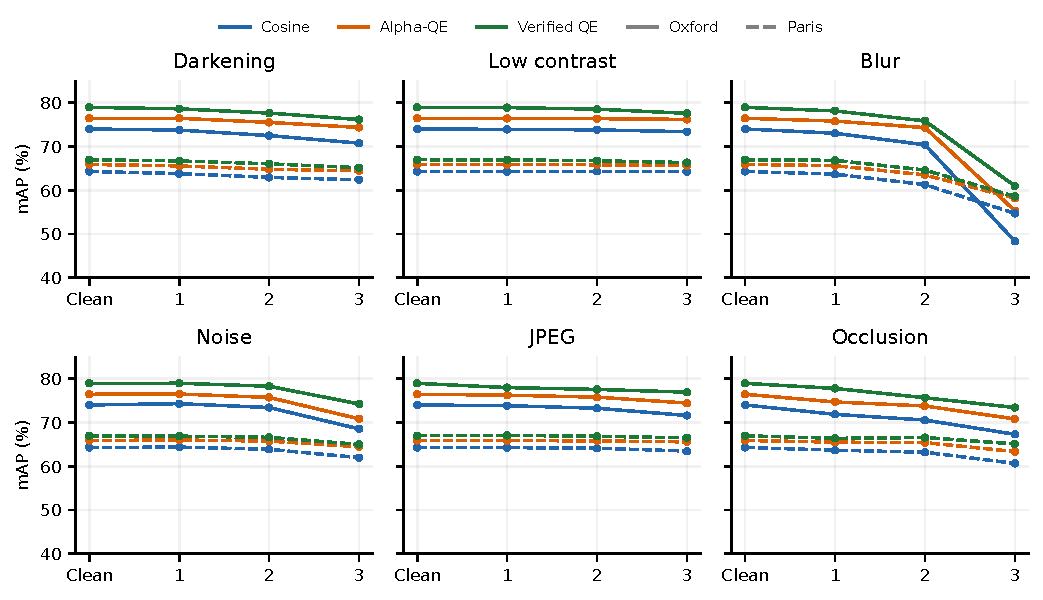
\includegraphics[width=0.96\textwidth]{robustness.pdf}
\caption{R1 retrieval under increasing query corruption. Solid curves: Oxford; dashed: Paris. Blue: cosine; orange: weighted QE; green: verified QE. Each non-clean point averages the prescribed realizations. The gallery is always clean.}
\label{fig:robustness}
\end{figure*}

Figure~\ref{fig:robustness} shows that severe blur is particularly damaging to \Rone. Its worst condition is blur severity three on both datasets: cosine mAP is 48.33\% Oxford and 54.71\% Paris. Verified QE raises those same condition scores to 60.97\% and 58.60\%, respectively. Improvements remain conditional on the starting encoder and the particular query transformations. A smaller clean-to-corrupted drop alone would not demonstrate a better system if absolute mAP were lower.

The suite partially overlaps training augmentation but is not identical. In particular, Gaussian noise is not included in the saved augmentation policy. Severe occlusion may remove identifying object content, and we do not claim that every generated query preserves perfect semantic observability. Results measure this defined stress test, not all natural distribution shifts.

Clean sensitivity contains 100 additional grouped evaluations, representing 5,500 per-query AP values. For instance, \Rone{} weighted QE with $\lambda=1$ reaches 77.30\% Oxford and 66.56\% Paris clean, above the frozen $\lambda=0.5$ setting. Local re-ranking with $K=100$ and $\eta=0.5$ reaches 78.85\% and 66.94\%. These are test-set observations, not independently validated parameter selections. They do not replace the main setting for corruption results. The complete configurations, including weaker variants, accompany the paper.

\subsection{RQ3: Quality--Latency Trade-offs}
\begin{figure*}[t]
\centering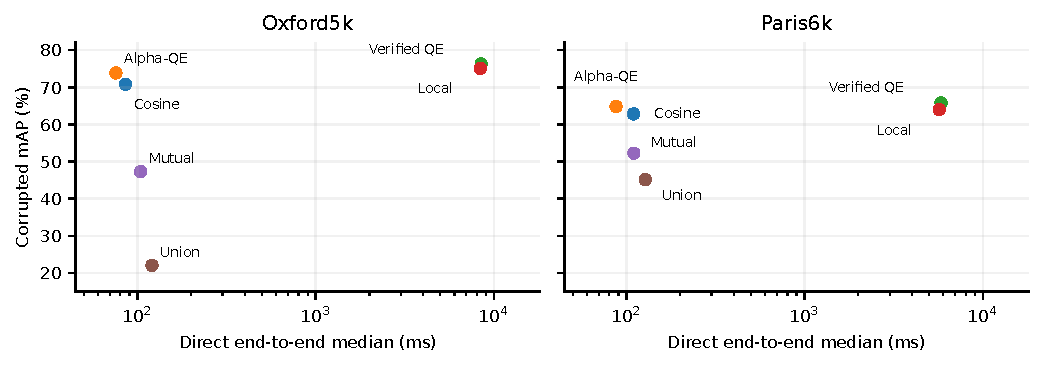
\includegraphics[width=0.96\textwidth]{quality_latency.pdf}
\caption{R1 corrupted mAP versus measured direct end-to-end median query latency (logarithmic horizontal axis). Quality uses the complete corruption suite; latency uses the predefined 28-sample subset. Offline gallery preparation is excluded.}
\label{fig:latency}
\end{figure*}

QE adds approximately 3--5 ms to retrieval-only processing for \Rone. Direct weighted-QE medians are 75.55 ms on Oxford and 87.34 ms on Paris. Verified QE has medians 8.48 s and 5.82 s; local matching and geometric processing dominate this scale of cost. These methods occupy substantially different deployment regimes (Fig.~\ref{fig:latency}).

The direct cosine medians for \Rone{} are 85.52 and 109.53 ms, larger than the corresponding weighted-QE medians despite QE's additional operation. The small, independently timed sample and execution variability prevent interpreting this ordering as a causal speed-up. Retrieval-only timings more directly expose the expansion overhead. We do not infer a speed improvement from the direct-median inversion.

Offline computation also matters. The shared local-feature cache reports approximately 2.56 GB of stored data. Its recorded builds take 2,464 s for Oxford and 3,049 s for Paris, covering gallery and query-view features. Query local features are nevertheless recomputed in the direct timer so cached queries do not hide online costs. Both fusion encoders must also be executed: direct score-fusion medians are 147.17 ms Oxford and 160.30 ms Paris. Its extra encoding cost does not yield an accuracy improvement here.

\subsection{Reproducibility and Limits of Inference}
The main grid has 20 ranking configurations per dataset: nine per encoder and two fusion rules. Across 110 queries and 31 views this yields 68,200 main AP records, with no missing cells in the saved coverage audit. Together with sensitivity, the saved per-query records total 73,700. Descriptors, rankings, image IDs, pixel checksums, checkpoint hashes, graph diagnostics, and job completion states identify the evaluated artifacts. Smoke checks cover export/reload consistency, finite descriptors, perfect/junk evaluator cases, QE identity and closed-gate behavior, single-ranker fusion, prefix-preserving re-ranking, and graph numerical behavior.

Only one training seed is available. The many corrupted views do not estimate variability across independent training runs, and we make no statistical-significance claim. Closely related landmark queries further limit interpretations based on treating all query views as independent observations. B0 lacks a matching corruption/post-training experiment, and the training histories differ in budget, precision, and runtime. Thus, the evidence supports fixed-encoder search gains and descriptive training observations, not a controlled attribution of gains or losses to augmentation or attention.

\section{Conclusion}
This study separates historical training observations from search-time improvements in VGG16--GeM retrieval. The validation-selected B0 remains a strong baseline, while the two new training runs exhibit late validation deterioration. On the completed B0 corruption study, AQE raises dataset-macro mAP from 77.20\% to 80.64\%. Sparse diffusion reaches 83.31\%, with a strong Paris gain but a clean Oxford loss. The same method therefore benefits some encoder/dataset combinations more than others.

An independent implementation audit identifies dense query seeding as the cause of the severe archived diffusion collapse. Correct seed support recovers useful rankings, yet it does not make diffusion uniformly beneficial. Archived local/geometric experiments also show that feedback quality and query cost matter: verified expansion improves the weaker epoch-100 encoders but costs seconds per query. Validation-based checkpoint selection, faithful implementation and separate quality/latency accounting are necessary for useful comparisons. The released source, numerical records and solver checks make these findings traceable.

\bibliographystyle{IEEEtran}
\bibliography{references}
\end{document}
